% ju 28-Mai-22
\documentclass[a4paper,12pt,fleqn,parskip=half]{scrartcl}
\usepackage[ngerman]{babel}
\usepackage[utf8]{inputenc}
\usepackage[T1]{fontenc}

% Schrift
%\usepackage{lmodern}
\usepackage[osf,sc]{mathpazo} 
\usepackage[scale=.9,semibold]{sourcecodepro}   
\usepackage[osf]{sourcesanspro}  

\usepackage[headsepline]{scrlayer-scrpage}
\pagestyle{scrheadings}
\clearpairofpagestyles

\usepackage[table,dvipsnames,usenames]{xcolor}
\usepackage{textcase}
\usepackage{nameref}
\usepackage{hyperref}
\usepackage{tabularx}
\usepackage{multirow}
\usepackage{multicol}
\usepackage{caption, booktabs}
\usepackage{graphicx} 
\usepackage{scrhack}    
\usepackage{url}%% Links
\usepackage[inline]{enumitem}
\usepackage{pifont}
\usepackage{eurosym}% \euro 20,-
\usepackage{amsmath}
\usepackage{amsfonts}
\usepackage{amssymb}
\usepackage{array}            % Extending the array and tabular environments
\usepackage{chngcntr}         % Change the resetting of counters
\usepackage[version=4]{mhchem}
\usepackage{stmaryrd}
\usepackage{siunitx}
\usepackage{float}
\usepackage{csquotes}
\usepackage{subcaption}
\usepackage{mathtools}
\usepackage{icomma}%Dezimaltrennzeichen
\usepackage{multimedia}%Video: \movie[externalviewer]{(video.mov)}{video.mov}
\usepackage{epstopdf}
\usepackage{footnote}
\usepackage{qrcode}% Anwendung: \qrcode[hyperlink,level=Q,version=2,height=1cm]{\website}
\usepackage{underscore}% Unterstrich ____

% PDF Dokumente einbinden
\usepackage{pdfpages}% \includepdf[pages=-]{Tabellen/Excel.pdf}
\RequirePackage{lastpage}  % Pagecounter

\addto\captionsngerman{%
\renewcommand{\figurename}{Abb.}
\renewcommand{\tablename}{Tab.}
}

% listings
\usepackage{listings}
\lstset{basicstyle=\linespread{1}\ttfamily\small,floatplacement=!htb,captionpos=t,abovecaptionskip=.5\baselineskip,belowcaptionskip=.5\baselineskip,upquote=true,showstringspaces=false,inputencoding=utf8,tabsize=4,
    	keywordstyle=\bfseries ,
	commentstyle=\color{rot5},
	stringstyle=\color{orange},
	breaklines=true,
  	postbreak=\mbox{\textcolor{black}{$\hookrightarrow$}\space},
	breakatwhitespace=false
}
\lstset{literate={á}{{\'a}}1 {é}{{\'e}}1 {í}{{\'i}}1 {ó}{{\'o}}1 {ú}{{\'u}}1 {Á}{{\'A}}1 {É}{{\'E}}1 {Í}{{\'I}}1 {Ó}{{\'O}}1 {Ú}{{\'U}}1 {à}{{\`a}}1 {è}{{\`e}}1 {ì}{{\`i}}1 {ò}{{\`o}}1 {ù}{{\`u}}1 {À}{{\`A}}1 {È}{{\'E}}1 {Ì}{{\`I}}1 {Ò}{{\`O}}1 {Ù}{{\`U}}1 {ä}{{\"a}}1 {ë}{{\"e}}1 {ï}{{\"i}}1 {ö}{{\"o}}1 {ü}{{\"u}}1 {Ä}{{\"A}}1 {Ë}{{\"E}}1 {Ï}{{\"I}}1 {Ö}{{\"O}}1 {Ü}{{\"U}}1 {â}{{\^a}}1 {ê}{{\^e}}1 {î}{{\^i}}1 {ô}{{\^o}}1 {û}{{\^u}}1 {Â}{{\^A}}1 {Ê}{{\^E}}1 {Î}{{\^I}}1 {Ô}{{\^O}}1 {Û}{{\^U}}1 {œ}{{\oe}}1 {Œ}{{\OE}}1 {æ}{{\ae}}1 {Æ}{{\AE}}1 {ß}{{\ss}}1 {ű}{{\H{u}}}1 {Ű}{{\H{U}}}1 {ő}{{\H{o}}}1 {Ő}{{\H{O}}}1 {ç}{{\c c}}1 {Ç}{{\c C}}1 {ø}{{\o}}1 {å}{{\r a}}1 {Å}{{\r A}}1 {€}{{\EUR}}1 {£}{{\pounds}}1 {~}{{\textasciitilde}}1 {-}{{-}}1 }

% bibliography
\usepackage[
    bibencoding=utf8,
    backend=biber,% bibtex, biber
    backref=false,backrefstyle=three+,url=true,urldate=comp,abbreviate=false,maxnames=20
]{biblatex} %Paket laden
\DeclareBibliographyCategory{cited}
\let\defaultcite\cite\renewcommand*\cite[2][]{\addtocategory{cited}{#2}\defaultcite[#1]{#2}}
\let\defaulttextcite\textcite\renewcommand*\textcite[2][]{\addtocategory{cited}{#2}\defaulttextcite[#1]{#2}}
\setcounter{biburllcpenalty}{7000}
\setcounter{biburlucpenalty}{8000}
\AfterPackage{biblatex}{
	\PreventPackageFromLoading[\errmessage{Sie haben versucht, das Cite-Paket zu laden, das nicht mit biblatex kompatibel ist.}]{cite}
}

\hypersetup{%
	%pdftitle={\titel},
	%pdfsubject={Latex},
	%pdfauthor={\autor},
	%pdfcreator={\autor}, 
	bookmarksnumbered=true,
	breaklinks=true,
	%colorlinks=true,	   
	linkcolor=rot5,		
	filecolor=blau5,		
	urlcolor=blau5,			
	citecolor=ForestGreen
}

\linespread{1.1}
\setlist{itemsep=0pt}
\widowpenalty10000
\clubpenalty10000
\tolerance1000   

\usepackage[left=2cm,right=2cm,top=1cm,bottom=1cm,includeheadfoot]{geometry}
%\usepackage[left=4cm,right=2cm,top=1cm, bottom=1cm,includeheadfoot]{geometry}
%\usepackage[left=6cm,right=1cm,top=1cm, bottom=1cm,includeheadfoot]{geometry}
%\usepackage[landscape=true,left=2cm,right=2cm,top=1cm,bottom=1cm,includeheadfoot]{geometry}%quer

% eigene Farbe definieren
% Adobe Prozessfarben: CMYK: 100,50,0,35 -> 1,0.5,0,0.35
\definecolor{orange}{cmyk}{0,0.55,0.61,0}   % 0,55,61,0
\definecolor{blau5}{cmyk}{1,0.77,0.1,0.01}  % 100,77,10,
\definecolor{rot5}{cmyk}{0.22,1,1,0.19}     % 22,100,100,19
\definecolor{grau2}{cmyk}{0,0,0,0.1}        % 0,0,0,40
\definecolor{blau}{cmyk}{0.93,0.66,0,0.21}% 

% Literatur
\bibliography{content/literatur}
\bibliography{content/literatur-kfz}
\bibliography{content/literatur-sport}

%%%%%%%%%%%%%%%%%%%%%%%%%%%%%%%%%%%%%%%%%%%%%%%%%%%%%%%
\newcommand{\name}{Jan Unger}% anpassen!!!!!
\newcommand{\thema}{FT_U10_VW_Stromlaufplan_Beleuchtungssystem_Loesung}% anpassen!!!!!
\newcommand{\quelle}{\name}
\newcommand{\website}{https://bw-ju.de/}
\newcommand{\github}{https://github.com/ju1-eu}
%%%%%%%%%%%%%%%%%%%%%%%%%%%%%%%%%%%%%%%%%%%%%%%%%%%%%%%

\ihead{\textbf{Quelle:} \quelle}%{Kopfzeile innen}
\ohead{\textbf{Datum:} \today}  %{Kopfzeile außen}

\ifoot{\textbf{Thema:} \thema}  %{Fußzeile  innen}
\ofoot{Seite {\thepage} von {\pageref{LastPage}}}%{Fußzeile  außen}

\title{\thema}
\author{\name}
\date{\today}

\begin{document}
	%\thispagestyle{empty}
	%\maketitle
	%\newpage
	%\setcounter{page}{1}

	%%%%%%%%%%%%%%%%%%%%%%%%%%%%%%%%%%%%%%%%%%%
	\begin{center}
		\textbf{\Large \thema}%14pt
		\vspace{0.8em}
		
		%\datum	
		%\qrcode[hyperlink,level=Q,version=2,height=1cm]{\website}
		\qrcode[hyperlink,level=Q,version=2,height=1cm]{\github}
	\end{center}
	%%%%%%%%%%%%%%%%%%%%%%%%%%%%%%%%%%%%%%%%%%%

	\subsection*{Keywords}%\label{sec:Deadline}\index{Deadline}
	% Checkliste
	\begin{itemize}[label=\checkmark] %\itemsep -2pt
		\item Begriff 
	\end{itemize}

    %%%%%%%%%%%%%%%%%%%%%%%%%%%%%%%%%%%%%%%%%%%%%%%%%%%%%%%%%%%%%%%%%%

	% anpassen
	%\input{content/tex/neu}
	%ju 28-Mai-22 FT_U10_VW_Stromlaufplan_Beleuchtungssystem_Loesung.tex
\section{Übungsaufgaben
Beleuchtungssystem}\label{uebungsaufgaben-beleuchtungssystem}

\textbf{(Ü10) Scheinwerferhöhenverstellung Beleuchtungssystem + VW
Stromlaufplan}

\textbf{Aufgabe 1}

\begin{itemize}
\item
  Ist eine Wartung durchgeführt worden?
\item
  Ist die Glühlampe oder der Scheinwerfer gewechselt worden
\item
  ist eine Motorwäsche durchgeführt worden
\item
  unter welchen Bedingungen ist dieses Ereignis aufgetreten
  (Feuchtigkeit, Wetter)
\item
  Unfall (Quetschung der Leitungen, Übergangswiderstand bilden)
\item
  witterungsbedingte Einflussnahme
\end{itemize}

\textbf{Aufgabe 2} Messung Strompfad 186-196 (Schaltplan VW -
Scheinwerferhöhenverstellung Beleuchtungssystem)

\begin{figure}[!ht]% hier: !ht
\centering
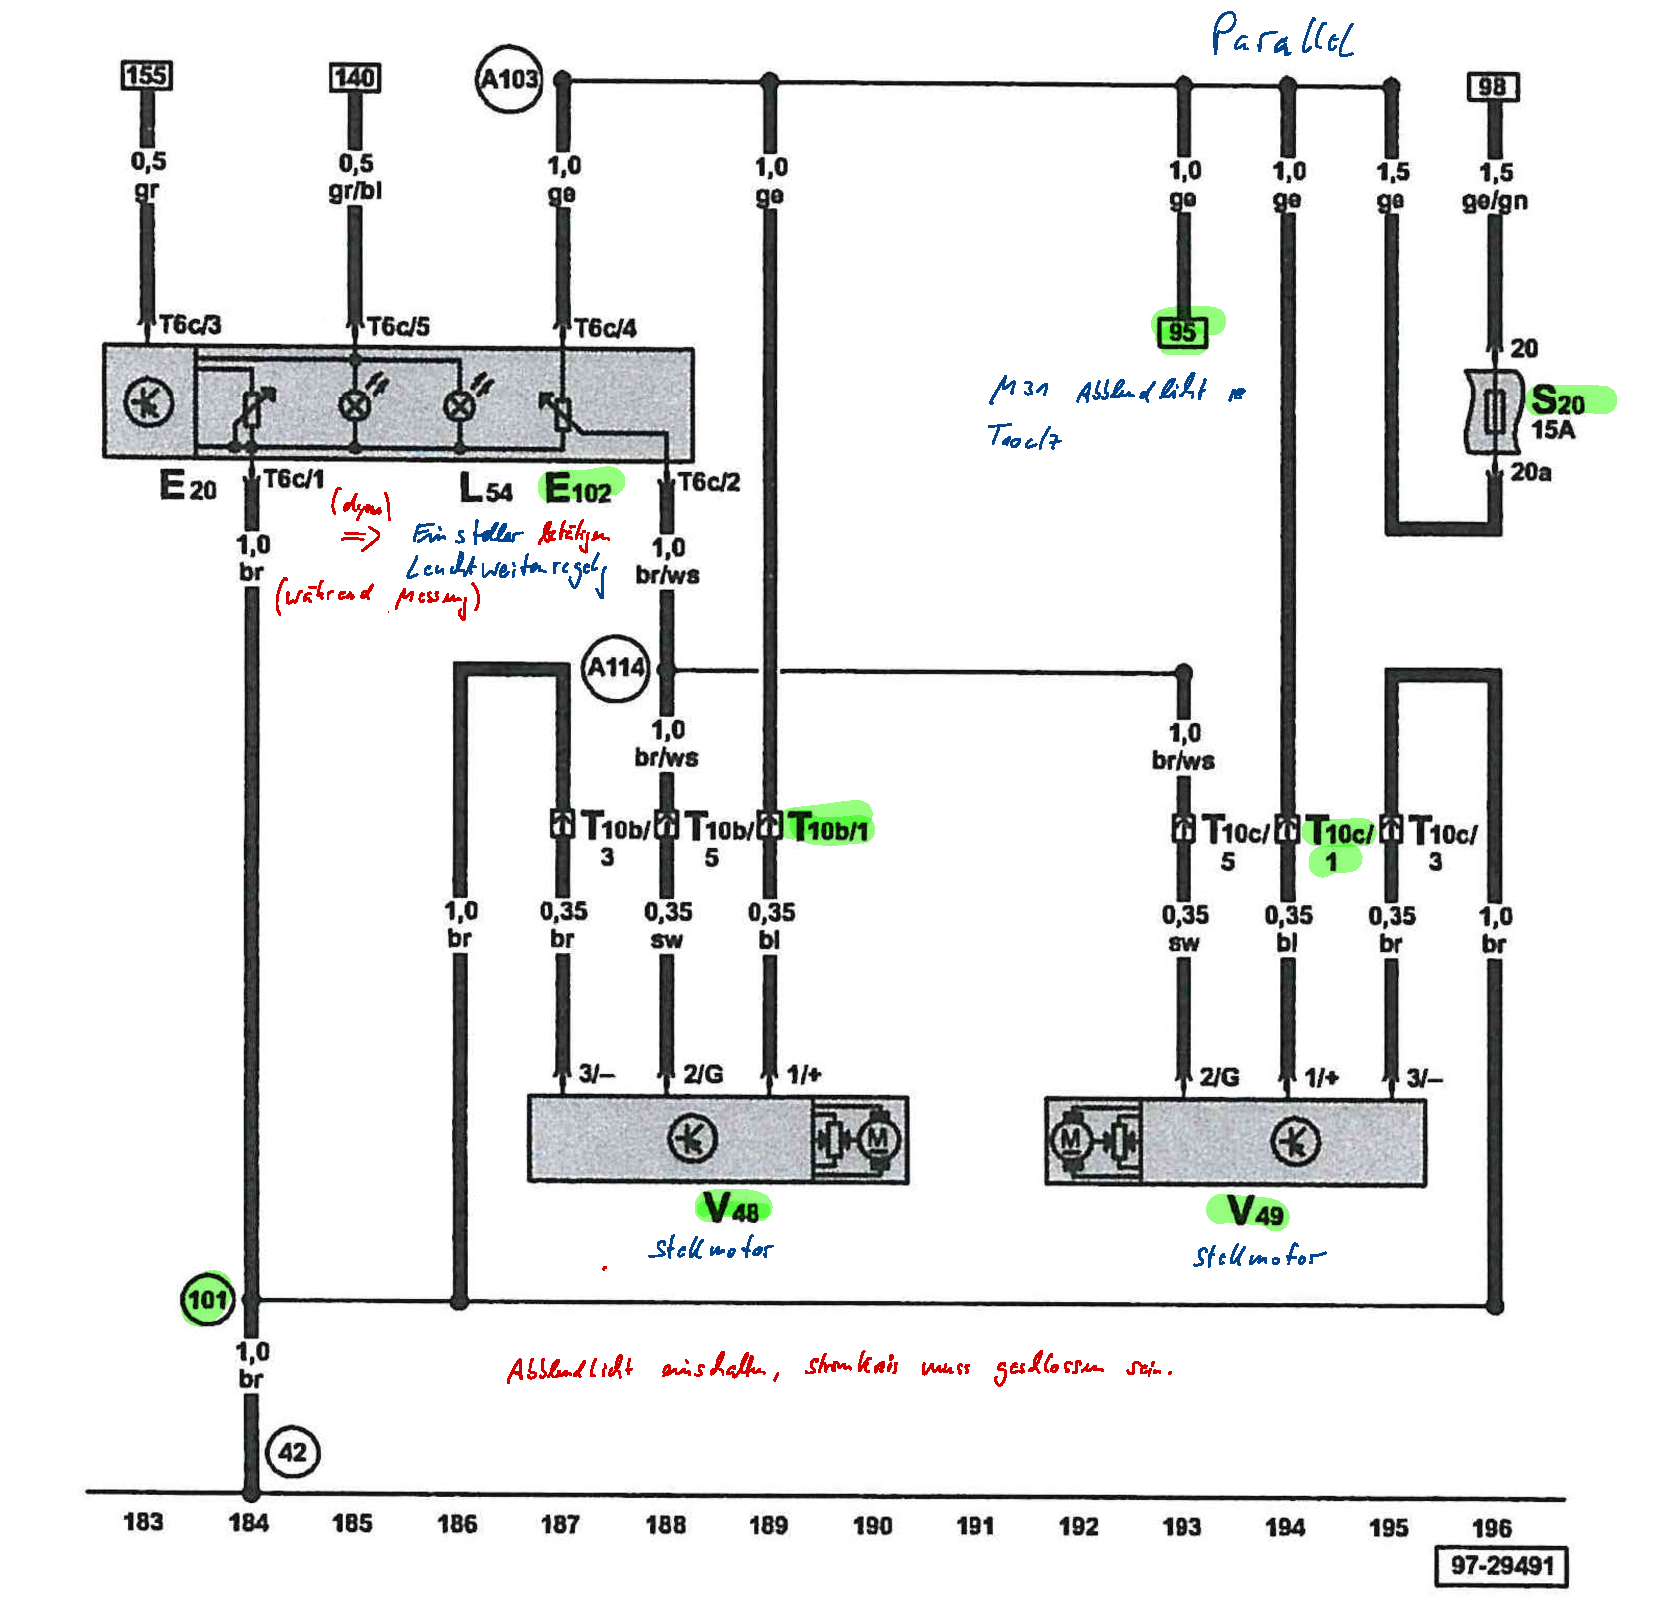
\includegraphics[width=0.9\textwidth]{images/Skizze/28_Scheinwerferhoehenverstellung.pdf}
\caption{Scheinwerferhöhenverstellung}
%\label{fig:}%% anpassen
\end{figure}

\begin{itemize}
\item
  Klemmenspannung Stellmotor messen
\item
  Geberspannung Signal (hoch/runter) messen
\item
  Synchronisierung der Höhenverstellung durchführen
\item
  mit Diagnosetester Fehlerspeicher auslesen
\item
  Sichtprüfung Stecker, Leitung, Sicherung, Mechanik
\end{itemize}

\textbf{Aufgabe 3} Ausgangszustand ist eine abgeglichene
Brückenschaltungsspannung zwischen dem Potenziometer E102 und
Potenziometern der Scheinwerfermotoren V48 und V49. Wird die
Potentiometerstellung (Stellrad) an E102 geändert, ändert sich
automatisch die Brückenspannung zwischen den beiden Komponenten \{E102
und den Potis von V48 und V49\}.

Die Auswerteelektronik erfasst im Brückenspannungswert und steuert die
Motoren V48 und V49 so lange mit der entsprechenden Polarität an, bis
die Brückenspannung wieder den Wert Null Volt erreicht. Die
Brückenspannung hat jetzt wieder ihren Ausgangswert (0 V), allerdings
bei einer anderen Stellung der Reflektoren.

Als Information über den Drehwinkelstand der Motoren, dienen die
Potenziometer, deren Schleifer mit den Reflektoren verbunden sind.

Das Bauteil, welches in der Regel verstellt wird, ist der Reflektor.

Die Drehrichtungsänderung erfolgt über die Polaritätsänderung an den
elektrischen Anschlüssen der Motoren.

\textbf{Aufgabe 4} Messobjekt (Poti E102) muss aus dem Stromkreis gelöst
und spannungsfrei sein.

Zur Messung des Wiederstandes Poti gemäß seiner Funktion
bewegen/drehen/verändern alle Funktionen/Stufen durchschalten.

\textbf{Aufgabe 5} Fahrzeuge mit Xeon Scheinwerfersystemen müssen mit
einer

\begin{enumerate}
\item
  automatischen Scheinwerferhöhenverstellungeinrichtung und
\item
  mit einer Scheinwerferreinigungsanlage ausgestattet sein,
\item
  bei Scheinwerfern mit Gasentladungslampen für Abblendlicht, wenn
  hierbei das Fernlicht eingeschaltet wird, muss das Abblendlicht in
  Funktion bleiben, also eingeschaltet bleiben
\end{enumerate}

siehe §50 STVZO, Tabellenbuch D2S, D2R, D1S, D1R

Scheinwerferhöhenverstellung

\begin{itemize}
\item
  Manuell
\item
  Automatisch
\item
  Dynamisch
\item
  Stichwort: Scheinwerferreinigungsanlage
\end{itemize}

\textbf{Aufgabe 6}

\begin{itemize}
\item
  Die Geräte M29, M31, V48 und V49 sind schaltungstechnisch parallel
  geschaltet, wobei M29 über die Sicherung S21 abgesichert wird,
  insofern hier keine Spannungsminderung auftreten wird
\item
  die Geräte M31 T10c/7, V48 T10b/1, V49 T10c/1, als auch E102 erfahren
  die Spannungsminderung um 3,25 V (alles auf die Masseversorgung des
  jeweiligen Bauteils gemessen)
\item
  Der Stromkreis muss geschlossen sein, es muss ein Strom fließen, also
  Licht (Abblendlicht) einschalten!
\item
  Einsteller E102 während der Messung betätigen
\end{itemize}

\textbf{Aufgabe 7}

Prüfzeichen und Bauartgenehmigung für Fahrzeugteile §21a, §22a

\begin{itemize}
\item
  \textbf{BRD} \verb|\~\~\~|
\item
  \textbf{EG} e1
\item
  \textbf{ECE} E1 (Prüfbuchstabe, Genehmigungsnummer, 1 = Deutschland, 2
  = Frankreich)
\end{itemize}

\textbf{Aufgabe 8}

Stromlaufplan Nr. 73/2 + 73/12 + 73/8 + 73/15

\begin{enumerate}
\item
  (Farbe Rot) Leuchtweitenregulierungsverlauf
\item
  (Farbe Blau) Laststrom Motoren Leuchtweiten
\item
  (Farbe Grün) Stromverlauf Abblendlicht
\end{enumerate}

\newpage

\textbf{Aufgabe 9}

Schaltbild

\begin{figure}[!ht]% hier: !ht
\centering
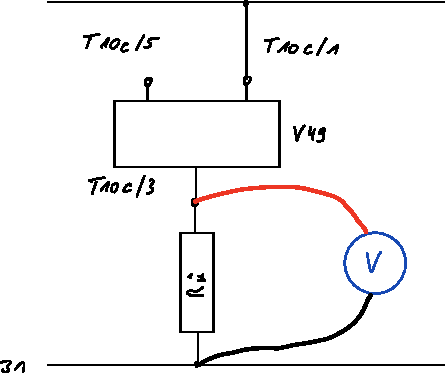
\includegraphics[width=0.6\textwidth]{images/Skizze/29_FT_minusseitiger_Ubergangswiderstand.pdf}
\caption{minusseitiger Übergangswiderstand}
%\label{fig:}%% anpassen
\end{figure}

Es hat sich zwischen T10c/3 und der Masseverbindung im Leitungsstrang
Strompfad 184 ein Übergangswiderstand gebildet, er liegt in Reihe zum
V49. Dieser Widerstand mindert die Klemmenspannung des Motors V49,
ferner bekommt die Brückenschalung des V49 unplausible Widerstandswerte.
Man spricht hierbei von einem minusseitigen Übergangswiderstand. Der
Spannungsverlust, der hierbei entsteht, bezeichnet man als einen
minusseitigen Spannungsverlust.

\begin{table}[!ht]% hier: !ht 
\centering 
	\caption{}% \label{tab:}%% anpassen 
\begin{tabular}{@{}ll@{}}
\hline
\textbf{Bezeichnung} & \textbf{Benennung} \\
\hline
V49 & Scheinwerferhöhenverstellmotor rechts \\
T10c/5 & Anschluss Steuerung \\
T10c/1 & Plusversorgung \\
T10c/3 & Masse \\
$R_\text{ü}$ & Übergangswiderstand \\
\hline
\end{tabular} 
\end{table}

\newpage

\textbf{Aufgabe 10}

\lstset{language=Python}% C, TeX, Bash, Python 
\begin{lstlisting}[
	%caption={}, label={code:}%% anpassen
][language=Python]
# geg:
P_M_31 = 55 W/12V
U = 12 # V
U_ges = 14,3 V
U_v = 3,25 V
# ges: P_M_31_tat
# Formel:
P_M_31 = U x I -> I = P_M_31 / U
R = U / I
I_tat = U_k / R -> I_tat = (U_ges - U_v) / R
P_M_31_tat = U_k x I_tat -> P_M_31_tat = (U_ges - U_v) x I_tat
# Lösung:
I = 4,5833 A
R = 2,6182 Ohm
I_tat = 4,2205 A
P_M_31_tat = 46,6364 W
\end{lstlisting}

\textbf{Aufgabe 11}

d = 31, 56a, 56b, 58R (Scheinwerfer vorne rechts)

\newpage

\textbf{Aufgabe 12}

\lstset{language=Python}% C, TeX, Bash, Python 
\begin{lstlisting}[
	%caption={}, label={code:}%% anpassen
][language=Python]
# geg:
P_12 = 21 W/12V
P_24 = 21 W/24V
U_12 = 12 V
U_24 = 24 V
# ges: R_24, R_12
# Formel:
P_12 = U x I -> I_12 = P_12 / U_12
R_12 = U_12 / I_12
P_24 = U x I -> I_24 = P_24 / U_24
R_24 = U_24 / I_24
Faktor = R_24 / R_12
# Lösung:
I_12 = 1,75 A
R_12 = 6,8571 Ohm
I_24 = 0,875 A
R_24 = 27,4286 Ohm
Faktor 12V / 24V = 4,0 -fache Leiterlaenge
\end{lstlisting}

Bei einer 24 V Glühlampe ist der Widerstand viermal größer (vierfache
Leiterlänge) als bei einer 12 V Glühlampe. Dieser Widerstand liegt
hierbei an einer doppelten Spannung gegenüber der 12 V Spannung. Durch
die doppelte Spannung und dem vierfachen Widerstand ergibt sich eine
gleiche Leistung, bei gleicher Baugröße des Glaskolbens. Um diesen
Widerstand in die gleiche Glaskolbengröße hineinzubekommen, ist die
Glühwendel mäanderförmig gefertigt, im Glaskolben verlegt.

\textbf{Aufgabe 13}

siehe Musterlösung


	%%%%%%%%%%%%%%%%%%%%%%%%%%%%%%%%%%%%%%%%%%%%%%%%%%%%%%%%%%%%%%%%%%
    % Bibliographie
    \printbibliography
\end{document}
